\documentclass{sis-dc}

\usepackage[utf8]{inputenc}

\usepackage{graphicx}
\graphicspath{{figures/}}
\usepackage{multirow} 
\usepackage{lipsum} % for lipsum blocks 
\usepackage{orcidlink} % for fancy orcidlink logos in title

% for definition environments
\usepackage{amsthm, amsmath}
%  definition environment
\theoremstyle{definition}
\newtheorem{defn}{Definition}

% defining some commands to shortcut notation
\newcommand{\universe}[1]{\mathcal{U}_{#1}} % shortcut for a universe
% defining some universes
\newcommand{\uacts}{\universe{\textit{act}}}
\newcommand{\utraces}{\universe{\mathcal{T}}}
\newcommand{\uevents}{\universe{\textit{ev}}}
\newcommand{\ucases}{\universe{\textit{case}}}
\newcommand{\uattrs}{\universe{\textit{att}}}
\newcommand{\udata}{\universe{\mathcal{D}}}
\newcommand{\uvalues}{\universe{\mathcal{V}}}
\newcommand{\utimes}{\universe{\Gamma}}
\newcommand{\umaps}{\universe{\textit{map}}}

% setup citing format and style
\usepackage{natbib}
\bibliographystyle{abbrvnat}
\setcitestyle{authoryear,open={(},close={)}}

% setup font and style for reference header
\renewcommand{\bibsection}{
    \setlength{\parskip}{18pt} 
    \par
    \noindent \fontsize{14pt}{14pt}\selectfont References
    \setlength{\parskip}{6pt}
    \par
}

\title{title of the paper}
\author{
Chih-Ping Wei \orcidlink{0000-0000-0000-0001}, Institute of Service Science, National Tsing Hua University, Hsinchu, Taiwan, R.O.C., cpwei@mx.nthu.edu.tw
% This is an example ORCID which is the right format, but not the number of any real scholar
\\
Han Zhang, College of Management, Georgia Institute of Technology, Atlanta, GA, USA, han.zhang@mgt.gatech.edu
\\
Patrick Y. K. Chau, School of Business, The University of Hong Kong, Hong Kong, pchau@business.hku.hk
}
\date{September 2021}

\begin{document}

% show authors
\maketitle[s]

% dont show authors
% \maketitle

\begin{abstract}
    \lipsum[3]
    
    \lipsum[5]
    
    Keywords: One, Two, Three, Four.
\end{abstract}

\clearpage

\section{Introduction}

\lipsum[1]

\subsection{In Depth Introduction}

\lipsum[2]

\begin{itemize}
    \item Studies into sucess factors have been conducted \citep{DBLP:journals/bpmj/BandaraGTR21}
    \item \cite{DBLP:journals/is/LeemansABP21}, \cite{DBLP:journals/kais/LeemansF20} and \cite{DBLP:conf/apn/BurkeLW21} are recent works from Dr. Sander J. J. Leemans.
\end{itemize}

\subsubsection{The Goods...}

\lipsum[3]
Here is a footnote\footnote{Congrats you have a free footnote for life}, quick take it and run.

\begin{figure}[t]
    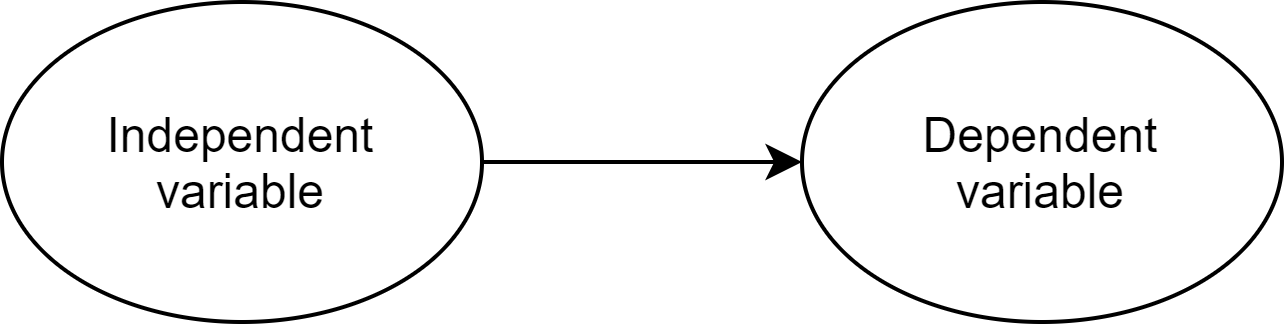
\includegraphics[width=0.6\textwidth]{sis-dc-example.png}
    \caption{ \lipsum[7] }
    \label{fig:my_label}
\end{figure}

\section{Theory}

To begin with, we define some universes (see Def. \ref{def:universe}) and then present our formalisation of an event log (see Def. \ref{def:eventlog}), but we acknowledge that other notations exist.

\begin{defn}[Universes]
$\udata = \{ \text{case},\text{act},\text{time}, \dots \}$ is the universe of data variables.
$\uvalues$ is the universe of values.
$\umaps = \udata \rightharpoonup \uvalues$ is the universe of variable to value mappings. 
$\uevents$ is the universe of events. 
\label{def:universe}
\end{defn}


\begin{defn}[Event Log]
An event log $\mathcal{E}$ is $(\text{E}, \pi)$, where $\text{E} \subseteq \uevents$ is a finite set of events, and $\pi : \uevents \rightarrow \umaps$ is a mapping from events to their attribute-value mappings.
\label{def:eventlog}
\end{defn}

\section{Results}

\begin{table}[b] %b for place at bottom, h for place here, t for place a top
\begin{tabular}{ |l|c|c| } 
\hline
\multicolumn{1}{|l|}{Question} &  \multicolumn{1}{|l|}{Average 1992} & \multicolumn{1}{|l|}{Average 1999} \\
\hline
 1 How do you regard... & 3.4 & 3.7 \\ 
 2 How do you... & 2.7 & 3.4 \\ 
 3 how do you... & 3.9 & 3.6 \\ 
 \hline
\end{tabular}
\caption{Experimental Results.}
\end{table}

\lipsum[5]

\begin{itemize}
    \item First-level bulleted list: foo bar foo foo foo some bar bar bar black sheep have any wool
    \begin{itemize}
        \item Second-level bullet list: foo foo foo some bar bar bar bar black sheep have any wool foo foo foo some bar bar bar bar black sheep have any wool
        \item Second-level bullet list: foo foo foo some bar bar bar bar black sheep have any wool foo foo foo some bar bar bar bar black sheep have any wool
        \item Second-level bullet list: foo foo foo some bar bar bar bar black sheep have any wool foo foo foo some bar bar bar bar black sheep have any wool
    \end{itemize}
    \item Another level one bullet point
\end{itemize}

foo foo foo some bar bar bar bar black sheep have any wool foo foo foo some bar bar bar bar black sheep have any woolfoo foo foo some bar bar bar bar black sheep have any wool foo foo foo some bar bar bar bar black sheep have any woolfoo foo foo some bar bar bar bar 
black sheep have any wool foo foo foo some bar bar bar bar black sheep have any woolfoo foo foo some bar bar bar bar black sheep have any wool foo foo foo some bar bar bar bar black sheep have any woolfoo foo foo some bar bar bar bar black sheep have any wool foo foo foo 
some bar bar bar bar black sheep have any wool.

foo foo foo some bar bar bar bar black sheep have any wool foo foo foo some bar bar bar bar black sheep have any woolfoo foo foo some bar bar bar bar black sheep have any wool foo foo foo some bar bar bar bar black sheep have any woolfoo foo foo some bar bar bar bar 
black sheep have any wool foo foo foo some bar bar bar bar black sheep have any woolfoo foo foo some bar bar bar bar black sheep have any wool foo foo foo some bar bar bar bar black sheep have any woolfoo foo foo some bar bar bar bar black sheep have any wool foo foo foo 
some bar bar bar bar black sheep have any wool

\bibliography{references/bib_refs.bib}

\end{document}
